\section{Data Aggregation}\label{aggregator}
As mentioned in Section~\ref{github}, I decided to use Github as my primary data source and to utilize their \emph{Github APIv3} for this purpose.
The aggregator and analysis program written for this thesis is named \emph{Gitalizer}.
In this section I will explain the technologies and methods used in the data aggregation process, the database structure and the interaction with Github's \ac{api}.
In the end some problems which occurred during the data collection will be shown as well.


\subsection{Existing Solutions}
There are of existing solutions for accessing and collecting git metadata.
In the following the practicability of these solutions will be evaluated based on our requirements.

\subsubsection{GHTorrent}
The \emph{GHTorrent} project aims to provide Github's metadata to elude the limitations Github's rate limiting~\cite{inproceedings:ghtorrent}.
It provides representations for followers and commits, as well as organizations and organization members, but there are some crucial informations missing.
GHTorrent only stores the main email address of a user and does thereby not support the handling of multiple emails, as commits are directly assigned to their respective Github user id.
Commits miss information about additions and deletions in lines of code, which implicates that each commit would need to be scanned by a separate program again.
Furthermore GHTorrent does not have the concept of \emph{starring}, which makes it hard to reduce the amount of repositories to scan to a manageable size.
Their database provides about 4~\ac{tb} of data according to their website, which is too much information without very precise limitation~\footnote{`The GHTorrent project' ghtorrent.com, http://ghtorrent.org/ (accessed, 05.05.2018)}
It provides a vast amount of data, but at the same time it cannot be ensure, that the data is as complete as possible for a specific user.
Modifying the GHTorrent code base and extending their database schema has thereby been judged as impractical.

\subsubsection{ghcrawler}
Microsoft provides an open-source crawler called \emph{ghcrawler}, which is supposed to continuously fetch data from Github~\footnote{`Github crawler' github.com, http://github.com/ (accessed, 05.05.2018)}.
Sadly their documentation is very bad and after diving into their source code, it appears that their crawler is for Github entities only and not for the underlying data of git repos.

\subsubsection{Alitheia-Core}
\emph{Alitheia-Core} is a Java data collector for git repositories.
It is not actively maintained since more than three years and their documentation website is offline.
Using this library seemed unpromising and unviable.

\subsubsection{RepoDriller}
The \emph{RepoDriller} project aims to support researchers by providing easy access to repository data from Github~\footnote{`A tool to support researchers on mining software repositories studies' github.com, http://github.com/ (accessed, 05.05.2018)}.
Despite providing a good solution for getting all necessary information from a repository, it provides no way to explore Github using \emph{stars} or \emph{following}.
These features, as well as assignment of emails to a contributor via the Github \ac{api}, would have to be added.
As the program is also written in Java and I am no longer familiar with the language and its ecosystem, I decided to stick to writing my own solution.

\subsection{Database}\label{gitalizer-database}
To store the gathered Information I chose a \ac{sql} based solution.
PostgreSQL provides excellent tools to ensure a high consistency in your database, namely check constraints, as well as great support for working with times, time zones and locations.
The \ac{sql} database is used in combination with the \ac{orm} library \emph{SQLAlchemy}.

The basic schema created for the purpose of this thesis consists of five \ac{orm} models.
A model for commits, emails, repositories, contributors and organizations has been created.
The latter is only important to validate results and is not actually used for knowledge discovery, as this is Github specific data.

\begin{figure}[H]
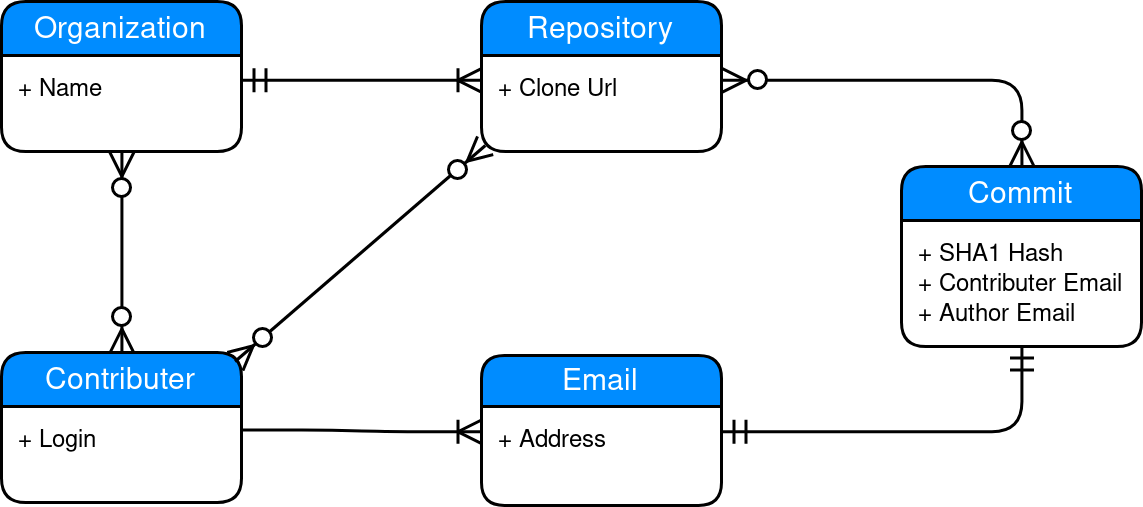
\includegraphics[scale=0.3]{./graphs/gitalizer-data-structure}
\centering
\caption{Gitalizer database relationships.}\label{fig:gitalizer-relationship}
\end{figure}

Every commit of each repository is saved in the database along with its \ac{sha1} hash and the two email addresses as in Listing~\ref{lst:raw-commit}.
It is important to note that there is a many-to-many relationship in figure~\ref{fig:gitalizer-relationship} between commits and repositories.
This feature prevents duplication of the same commits from forked repositories.
It is, for instance, a common practice to create a fork of a repository to develop without intervening with the main git repository of the project.
As described in Section~\ref{git-internal-representation} the probability of a \ac{sha1} collision is highly improbable.
By exploiting this feature, it is possible to enforce a unique constraint on the commit hash column, assuming that any duplicated commit hash actually results from a forked or copied repository.
The formula for calculating the probability of such a collision is as follows, where $p$ is the probability of collision, $n$ is the amount of different hashes and $b$ is the size of the hash in bytes:

\begin{equation}\label{eq:collision-probability}
    p \leq \frac{n(n-1)}{2} * \frac{1}{2^{b}}
\end{equation}

Without this mechanism it could be possible that the same commit of a contributor could be used multiple times as a result of repository forking.
After collecting 43 million commits from Github and actively ignoring obvious project forks, there are still 49 million references between commits and repositories.
This means that about 13\% of gathered commits result from forked repositories which can not easily be identified as such.
Considering Formula~\ref{eq:collision-probability}, the probability of a collision for 49 million hashes on the 160 bit \ac{sha1} hash would be about $8.21 * 10^{-34}$.

As stated above each commit is also saved with its respective email addresses.
There exists a one-to-many relationship between contributors and emails, as every contributor can obtain an unlimited amount of email addresses.
It is necessary to connect all email addresses commit to a specific contributor, to unambiguously assign all commit to their respective contributor.
This relationship does not have a \inlinecode{NOT NULL} constraint as it happens quite often that an email address can not be assigned to any person.
Looking at the collected data it appears that roughly 20\% of all collected email addresses from Github are no longer connected to an active user.

As stated in Section~\ref{github-features} Github provides a way to organize several people in organizations and teams.
As one of the goals of this thesis is to see if it is possible to detect member of an organization in open-source projects, a model for organization has been created as well.
This data can then be used to check against the results of this research's results.


\subsection{Gitalizer}
The Program written for this thesis features data aggregation, preprocessing, knowledge extraction and visualization.
Gitalizer uses a PostgreSQL database for data storage and data consistency checks as described in~\ref{gitalizer-database}.
For interaction with the Github \ac{api} the \emph{PyGithub} library is used, which provides a convenient abstraction layer for requests and automatically maps \ac{json} responses to \emph{Python} objects.

The data aggregation module of Gitalizer is capable of several approaches for gathering data.
In the following we will look at those approaches in detail.

\begin{description}
    \item[Git repository]\label{stand-alone-repository-scan} \hfill \\
        Gitalizer can scan any git repository from a \ac{ssh} or \ac{http} \acs{url} as long as the current user has access to it.
        The repository is cloned into a local directory. After the cloning finished the actual scanning process begins.
        During the scan, we git checkout the HEAD of the current default branch for this repository and walk down every reachable commit of the Git history.
        The program saves all available metadata for each commit in its database, namely the emails, timestamps as well as additions and deletions to the project in lines of code.

        After this scan we are still missing a lot of information.
        There exists no unique identifier of an author or committer, as names may change or can be ambiguous and a single person can have multiple email addresses.
        The problem with the simplicity of Git is that there exists no concept of an user.
        Thereby we cannot easily link several email addresses to a specific contributor without additional metadata.


    \item[Github Repository]\label{github-repo-scan} \hfill \\
        To tackle the problem of missing metadata in~\ref{stand-alone-repository-scan}, I used the Github \ac{api} to get some of the missing metadata.
        The general approach is the same as in the previous scan method. The repository is cloned and locally scanned.
        However, a request to Github is issued every time an email is found, which we do not already have linked to a contributor.
        Github allows to link multiple email addresses with a single user account and automatically references the respective user in their own \ac{api} commit representation.
        With this additional metadata we gain ground truth about the identity of an author or committer.

        Anyway this approach does not work, if the user of a commit removes the email, which has been used for the commit, from his account or if the user completely deletes their account.
        If this happens and the email contributor relationship has not already been created, there is nothing that can be done and these commits need to be handled later on in the preprocessing of the data.

    \item[Github User]\label{github-repo-scan} \hfill \\
        To try getting all repositories of a specific user, a new functionality has been added, which highly utilizes the Github \ac{api}.
        At first several requests are issued to get all repositories of the specified user, as well as all starred repositories of this user.
        During the repository exploration, every relevant repository is added to a shared queue, lets call it ``repo-queue'', which is then processed by a multiprocessing pool of workers.
        Each worker process pops another entry from the ``repo-queue'' and scans a single repository as described in~\ref{github-repo-scan}.


    \item[Connected users and organizations]\label{github-repo-scan} \hfill \\
        For detection and analysis of connections between contributors over multiple repositories additional user repository discovery as described in~\ref{requirements}, another feature has been added to Gitalizer.
        Gitalizer is able to achieve this by not just scanning a single user, but also scanning the repositories of all following and followed users as described in~\ref{github-user-scan}.
        For this task two different worker pools are utilized.
        The user discovery pool is initialized with a shared queue, lets call it ``user-queue'', of all users we need to look at.
        This worker pool simply searches for relevant repositories of each user and passes the repository \ac{url} to a second shared queue.
        The second pool then processes this ``repo-queue'' as described in~\ref{github-repo-scan}.

        For organizations it is nearly the same approach.
        Initially all repositories, which are owned by the organization, are added to the ``repo-queue''.
        All publicly visible organization members are then added to the ``user-queue'' and processed as described above.
\end{description}


\subsection{Database Optimization}
As the database kept growing, it became the bottleneck in the aggregation process several times.
As a result, adjustments in the database schema, PostgreSQL parameter tweaking and migration to better hardware were necessary.
The first considerable slowdown occurred after reaching about 12~\acp{gb} of data.
At this stage the database write and read operations took longer than the actual aggregation process and the whole machine started to become unresponsive because of high I/O load.

The performance of the database then needed to be continuously tweaked in several steps.
The first countermeasure was the reduction of commits using deduplication by using the features of the \ac{sha1} hash as stated in Section~\ref{database-design}
The ignoring of forked repositories reduced the amount of entries in the relation table between commits and repositories by another 26\%.

The next performance boosts were achieved by disabling or loosening several fail-safe mechanisms of PostgreSQL, namely `synchronous commit' and `write ahead' parameter, which are designed to save data on a system crash.
As there is no important or critical data handled it was acceptable to pass on these mechanisms, and trade safety for performance.

\begin{figure}[H]
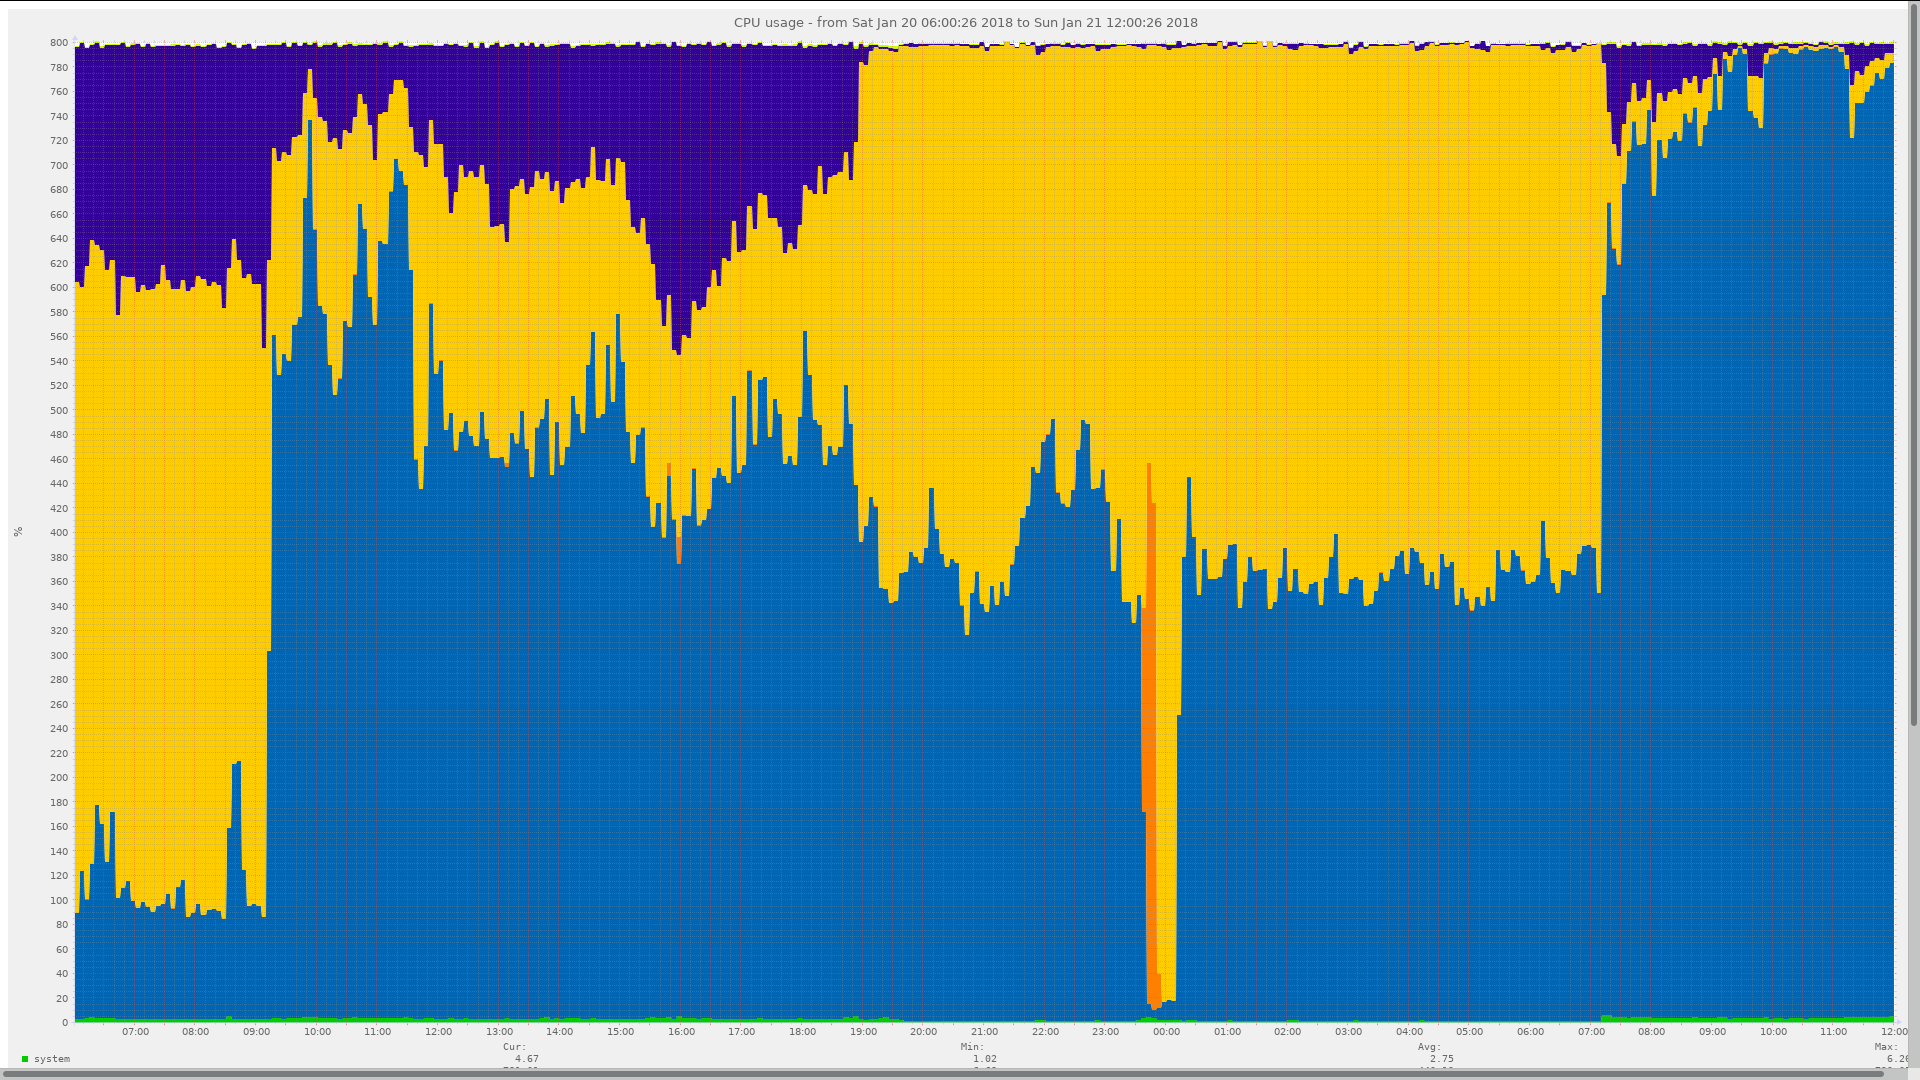
\includegraphics[scale=0.22]{./graphs/server-graphs/query-refactoring}
\centering
\caption{The CPU load of the aggregation server during optimization.}\label{fig:cpu-load}
\end{figure}

After renting a root server and deploying Gitalizer onto it, the aggregation process worked really well, until the database size hit about 25~\ac{gb}.
In Figure~\ref{fig:cpu-load} you see the overall CPU load right before optimizing several \ac{sql} queries by caching intermediate results and increasing the cache size of PostgreSQL.
The dark blue represents the I/O wait time while the light blue represents the actually used processor capacity by the aggregator.
Due to complex and numerous \ac{sql} queries the server became partly unresponsive and the aggregation process began to stall.

After many improvements the server can now run with 16 worker threads and roughly 38~\ac{gb} of data without any signs of slowdown whilst using the rate limit to capacity.


\subsection{Incremental Aggregation}
To ensure a constantly up to date database, Gitalizer needed to be capable of fast rescans of repositories.
The initial scan of a repository always includes cloning, scanning the whole repository and writing it into the database.
After a repository is scanned completely at least once it is marked as as such and will never by completely scanned again.
All following runs then only clone the repository and scan the newest unknown commits.
These are discovered by performing a breadth first search until no new nodes are found.

\begin{figure}[H]
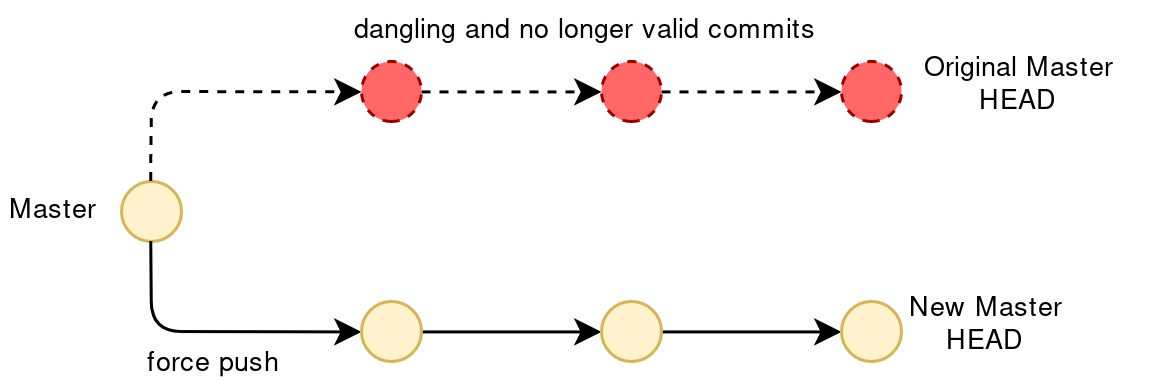
\includegraphics[scale=0.3]{./graphs/git-history-rewrite}
\centering
\caption{Gitalizer database relationships.}\label{fig:gitalizer-relationship}
\end{figure}

As explained in Section~\ref{more-git-features} it is possible to rewrite commits and force push them.
This scenario needs to be explicitly handled since force pushes can completely alter the history of a git repository, which can subsequently lead to a split in the Git history and leaves dangling commits.
As the complete history of a repository is stored inside the database, Gitalizer needs to detect a force push by walking down the git history tree until it finds known commits.
If any of these commits has children, which are not in the newly scanned commits, a force push took place and the old commit history has to be flagged, since it is now outdated and irrelevant.
An example scenario can be seen in Figure~\ref{fig:gitalizer-relationship}, where all red commits represent the old commit history, which needs to be truncated.


\subsection{Problems}
During the development of the data aggregator I experienced a few problems and edge cases which needed to be handled.
The earliest and most delaying problem was the rate limit of the Github \ac{api}, which limits to 5000 requests per hour.
Beside this rate limiting there also is an abuse detection mechanism, which triggers, if too many requests are fired in a short amount of time.
The solution for this problem resulted in various patches, which include random wait times to detain those mechanisms from triggering.

The first version of the aggregator did not clone and scan the repository locally, but rather gathered all information from the Github \ac{api} endpoints.
This approach worked well until the aggregator hit the official repository of \emph{Nmap}, which has about 11.000 commits and took over three hours to scan.
Soon I realized that this would severely slow down my research and I then started to continuously minimize the amount of \ac{api} calls issued by Gitalizer, to avoid waiting for a reset of the previously mentioned \ac{api} limit.
A connected user scan of my own Github account led to about 600.000 commits and took about one and a half day on the final working version of Gitalizer, to provide you with a reference of scale.

After implementing multiprocessing, I managed to hit the rate limit again, as I was now issuing requests to the \ac{api} with multiple threads.
To fix this issue I implemented a wait and retry wrapper around every single function call or object access, which triggered a call to the Github \ac{api}.
Afterwards the aggregator was capable of running multiple days without worker processes silently dying or finishing with incomplete data.

Fine tuning the edge cases and the handling of the \ac{api} took about 3 months, since there were many problems such as unpredictable error responses from Github, missing data in queries or simply unknown or broken encodings in Github's metadata.

A big throwback became apparent as I discovered that PostgreSQL automatically normalizes \ac{utc} timestamps with any offset to the \inlinecode{UTC +0} timezone.
As a result of this normalization, the exact time of the commit admittedly stays the same, but the crucial metadata about the offset is lost.
As a consequence the commit model needed to be adjusted, as the \ac{utc} offset had to be stored explicitly, and the whole commit aggregation process was started from scratch.

Another problem occurred during the local scanning of the repositories.
The library used for interaction with Git \emph{libgit2} issued \emph{stat} Linux syscalls during a diff operation for each file, which changed between those commits, to check if there were any local uncommitted changes.
Anyhow the repositories, which were locally scanned, were cloned with \emph{bare} mode.
This means that there exists no project root directory, but rather only the git internal representations of those files, which makes the behaviour stated above unnecessary and unwanted.
As a result all processes slowed severely down due to high I/O wait times, because of stat syscalls on non existent files.
Luckily after reporting the issue~\footnote{`Unnecessary syscalls on bare repository' github.com, https://github.com/libgit2/libgit2/issues/4480 (accessed, 25.04.2018)} it was resolved in a week and I was able to continue developing with my own compiled version of the libgit2 library.
